    %iffalse
                        \let\negmedspace\undefined
                        \let\negthickspace\undefined
                        \documentclass[journal,12pt,twocolumn]{IEEEtran}
                        \usepackage{cite}
                        \usepackage{amsmath,amssymb,amsfonts,amsthm}
                        \usepackage{algorithmic}
                        \usepackage{graphicx}
                        \usepackage{textcomp}
                        \usepackage{xcolor}
                        \usepackage{txfonts}
                        \usepackage{listings}
                        \usepackage{enumitem}
                        \usepackage{mathtools}
                        \usepackage{gensymb}
                        \usepackage{comment}
                        \usepackage[breaklinks=true]{hyperref}
                        \usepackage{tkz-euclide} 
                        \usepackage{listings}
                        \usepackage{gvv}                                        
                        %\def\inputGnumericTable{}   
                        \renewcommand{\thetable}{\theenumi}
                        \usepackage[latin1]{inputenc}                                
                        \usepackage{color}                                            
                        \usepackage{array}                                            
                        \usepackage{longtable}                                       
                        \usepackage{calc}                                             
                        \usepackage{multirow}                                         
                        \usepackage{hhline} 
                        \usepackage{tikz}
                        \usepackage{ifthen}                                           
                        \usepackage{lscape}
                        \usepackage{tabularx}
                        \usepackage{array}
                        \usepackage{float}
                        \newtheorem{theorem}{Theorem}[section]
                        \newtheorem{problem}{Problem}
                        \newtheorem{proposition}{Proposition}[section]
                        \newtheorem{lemma}{Lemma}[section]
                        \newtheorem{corollary}[theorem]{Corollary}
                        \newtheorem{example}{Example}[section]
                        \newtheorem{definition}[problem]{Definition}
                        \newcommand{\BEQA}{\begin{eqnarray}}
                        \newcommand{\EEQA}{\end{eqnarray}}
                        \theoremstyle{remark}
                        % Marks the beginning of the document
                        \begin{document}
                        \bibliographystyle{IEEEtran}
                        \vspace{3cm}
                        \title{2009-ME-'49-60'}
                        \author{AI24BTECH11006 - Bugada Roopansha}
                        \maketitle
                        \begin{enumerate}[start=49]
 \item What are the upper and lower limits of the shaft represented by $60 \, f_8$?
    
    Use the following data:
    \begin{itemize}
        \item Diameter $60$ lies in the diameter step of $50 - 80$ mm.
        \item Fundamental tolerance unit, $i$, in $\mu$m = $0.45 \brak{D^{1/3}} + 0.001 D$, where $D$ is the representative size in mm.
        \item Tolerance value for $IT8 = 25i$.
        \item Fundamental deviation for `$f$` shaft $= -5.5 D^{0.41}$.
    \end{itemize}
    
    \begin{enumerate}
        \item Lower limit $= 59.924$ mm, Upper limit $= 59.970$ mm
        \item Lower limit $= 59.954$ mm, Upper limit $= 60.000$ mm
        \item Lower limit $= 59.970$ mm, Upper limit $= 60.016$ mm
        \item Lower limit $= 60.000$ mm, Upper limit $= 60.046$ mm
    \end{enumerate}
    
    \item Match the items in Column I and Column II.
    
    \begin{table}[h!]
        \centering
        \begin{tabular}{|c|l|}
            \hline
            \textbf{Column I} & \textbf{Column II} \\
            \hline
            Metallic Chills & Support for the core \\
            \hline
            Metallic Chaplets & Reservoir of the molten metal \\
            \hline
            Riser & Control cooling of critical sections \\
            \hline
            Exothermic Padding & Progressive solidification \\
            \hline
        \end{tabular}
    \end{table}
    
    \begin{enumerate}
        \item $P - 1, Q - 3, R - 2, S - 4$
        \item $P - 1, Q - 4, R - 2, S - 3$
        \item $P - 3, Q - 4, R - 2, S - 1$
        \item $P - 4, Q - 1, R - 2, S - 3$
    \end{enumerate}
  

  \section{  Common Data for Questions 51 and 52:}
    
    The inlet and outlet conditions of steam for an adiabatic steam turbine are as indicated in the figure. The notations are as usually followed.
    
    \begin{itemize}
        \item $h_1 = 3200 \, \frac{kJ}{kg}$
        \item $V_1 = 160 \, \frac{m}{s}$
        \item $Z_1 = 10 \, m$
        \item $P_1 = 3 \, MPa$
        \item $h_2 = 2600 \, \frac{kJ}{kg}$
        \item $V_2 = 100 \, \frac{m}{s}$
        \item $Z_2 = 6 \, m$
        \item $P_2 = 70 \, kPa$
    \end{itemize}

    \item If mass flow rate of steam through the turbine is $20 \, \frac{kg}{s}$, the power output of the turbine $\brak{in 
 MW}$ is
    \begin{enumerate}
        \item $12.157$
        \item $12.941$
        \item $168.001$
        \item $168.785$
    \end{enumerate}

    \item Assume the above turbine to be part of a simple Rankine cycle. The density of water at the inlet to the pump is $1000 \, \frac{kg}{m^3}$. Ignoring kinetic and potential energy effects, the specific work $\brak{in \frac{kJ}{kg}}$ supplied to the pump is
    \begin{enumerate}
        \item $0.293$
        \item $0.351$
        \item $2.930$
        \item $3.510$
    \end{enumerate}

   \section{ Common Data for Questions 53 and 54:}
    
    Radiative heat transfer is intended between the inner surfaces of two very large isothermal parallel metal plates. While the upper plate $\brak{designated as plate 1}$ is a black surface and is the warmer one being maintained at $727 $\degree C, the lower plate \brak{plate 2} is a diffuse and gray surface with an emissivity of $0.7$ and is kept at $227 $\degree C. Assume that the surfaces are sufficiently large to form a two-surface enclosure and steady-state conditions to exist. Stefan-Boltzmann constant is given as $5.67 \times 10^{-8} \, \frac{W}{{m}^2{K}^4}$.

\item The irradiation \brak{in \frac{\text{kW}}{\text{m}^2}} for the upper plate \brak{plate 1} is


    \begin{enumerate}
        \item $2.5$
        \item $3.6$
        \item $17.0$
        \item $19.5$
    \end{enumerate}

    \item If plate $1$ is also a diffuse and gray surface with an emissivity value of $0.8$, the net radiation heat exchange \brak{in \frac{\text{kW}}{\text{m}^2}} between plate $1$ and plate $2$ is
    \begin{enumerate}
        \item $17.0$
        \item $19.5$
        \item $23.0$
        \item $31.7$
    \end{enumerate} 

\section{ Common Data for Questions 55 and 56:}
    
    Consider the following PERT network:
    
   \begin{center}
    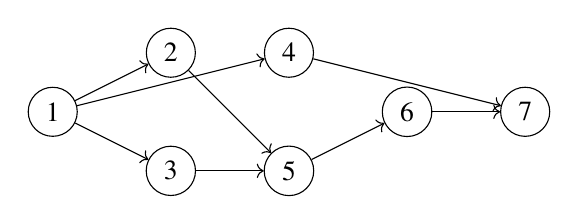
\begin{tikzpicture}[scale=0.75] % Removed the comma after tikzpicture
        % Example of a simple PERT diagram
        \node[circle, draw] (1) at (0,0) {1};
        \node[circle, draw] (2) at (2,1) {2};
        \node[circle, draw] (3) at (2,-1) {3};
        \node[circle, draw] (4) at (4,1) {4};
        \node[circle, draw] (5) at (4,-1) {5};
        \node[circle, draw] (6) at (6,0) {6};
        \node[circle, draw] (7) at (8,0) {7};

        \draw[->] (1) -- (2);
        \draw[->] (1) -- (3);
        \draw[->] (1) -- (4);
        \draw[->] (2) -- (5);
        \draw[->] (3) -- (5);
        \draw[->] (5) -- (6);
        \draw[->] (4) -- (7);
        \draw[->] (6) -- (7);
    \end{tikzpicture}
\end{center}

    The optimistic time, most likely time, and pessimistic time of all the activities are given in the table below:
    
    \begin{table}[h!]
    \centering
    \begin{tabular}{|p{2cm}|p{2cm}|p{2cm}|p{2cm}|} % Adjust the widths as needed
        \hline
        \textbf{Activity} & \textbf{Optimistic time \brak{days}} & \textbf{Most likely time \brak{days}} & \textbf{Pessimistic time \brak{days}} \\
        \hline
        1-2 & 1 & 2 & 3 \\
        1-3 & 5 & 6 & 7 \\
        1-4 & 3 & 5 & 7 \\
        2-5 & 5 & 7 & 9 \\
        3-5 & 2 & 4 & 6 \\
        5-6 & 4 & 5 & 6 \\
        4-7 & 4 & 6 & 8 \\
        6-7 & 2 & 3 & 4 \\
        \hline
    \end{tabular}
    
\end{table}

    \item The critical path duration of the network \brak{in days} is
    \begin{enumerate}
        \item $11$
        \item $14$
        \item $17$
        \item $18$
    \end{enumerate}

    \item The standard deviation of the critical path is
    \begin{enumerate}
        \item $0.33$
        \item $0.55$
        \item $0.77$
        \item $1.66$
    \end{enumerate}

    

   \section{ Statement for Linked Answer Questions 57 and 58:}
    
    In a machining experiment, tool life was found to vary with the cutting speed in the following manner:
    
    \begin{table}
    \centering
        \begin{tabular}{|c|c|}
            \hline
        \textbf{ Cutting speed \brak{\frac{m}{min}}} & \textbf{Tool life \brak{minutes}}\\
        \hline
        60 & 81 \\
        90 & 36 \\
        \hline
        \end{tabular}
    \end{table}
    
    \item The exponent ($n$) and constant ($k$) of the Taylor's tool life equation are
    \begin{enumerate}
        \item $n = 0.5$ and $k = 540$
        \item $n = 1$ and $k = 4860$
        \item $n = -1$ and $k = 0.74$
        \item $n = -0.5$ and $k = 1.155$
    \end{enumerate}
    \item  What is the percentage increase in tool life when the cutting speed is halved?
    \begin{enumerate}
        \item $50\%$
        \item $200\%$
        \item $300\%$
        \item $400\%$
    \end{enumerate}

\section{ Statement for Linked Answer Questions 59 and 60}
    
  \item   A $20$\degree full depth involute spur pinion of $4$ mm module and $21$ teeth is to transmit $15$ kW at $960$ rpm. Its face width is $25$ mm.

    \item  The tangential force transmitted \brak{in N} is
    \begin{enumerate}
        \item $3552$
        \item $2611$
        \item $1776$
        \item $1305$
    \end{enumerate}

    \item  Given that the tooth geometry factor is $0.32$ and the combined effect of dynamic load and allied factors intensifying the stress is $1.5$; the minimum allowable stress \brak{in MPa} for the gear material is
    \begin{enumerate}
        \item $242.0$
        \item $166.5$
        \item $121.0$
        \item $74.0$
    \end{enumerate}
\end{enumerate}





    

\end{document}
